\documentclass[12pt]{article}
\usepackage[left=1cm, right=1cm, top=2cm,bottom=1.5cm]{geometry} 

\usepackage[parfill]{parskip}
\usepackage[utf8]{inputenc}
\usepackage[T2A]{fontenc}
\usepackage[russian]{babel}
\usepackage{enumitem}
\usepackage[normalem]{ulem}
\usepackage{amsfonts, amsmath, amsthm, amssymb, mathtools}

\usepackage{tabularx}
\usepackage{hhline}

\usepackage{accents}
\usepackage{fancyhdr}
\pagestyle{fancy}
\renewcommand{\headrulewidth}{1.5pt}
\renewcommand{\footrulewidth}{1pt}

\usepackage{graphicx}
\usepackage[figurename=Рис.]{caption}
\usepackage{subcaption}
\usepackage{float}

%%Наименование папки откуда забирать изображения
\graphicspath{ {./images/} }

%%Изменение формата для ввода доказательства
\renewcommand{\proofname}{$\square$  \nopunct}
\renewcommand\qedsymbol{$\blacksquare$}

%%Изменение отступа на таблицах
\addto\captionsrussian{%
	\renewcommand{\proofname}{$\square$ \nopunct}%
}
%% Римские цифры
\newcommand{\RN}[1]{%
	\textup{\uppercase\expandafter{\romannumeral#1}}%
}

%% Для удобства записи
\newcommand{\MR}{\mathbb{R}}
\newcommand{\MC}{\mathbb{C}}
\newcommand{\MQ}{\mathbb{Q}}
\newcommand{\MN}{\mathbb{N}}
\newcommand{\MZ}{\mathbb{Z}}
\newcommand{\MTB}{\mathbb{T}}
\newcommand{\MTI}{\mathbb{I}}
\newcommand{\MI}{\mathrm{I}}
\newcommand{\MJ}{\mathrm{J}}
\newcommand{\MH}{\mathrm{H}}
\newcommand{\MT}{\mathrm{T}}
\newcommand{\MU}{\mathcal{U}}
\newcommand{\MV}{\mathcal{V}}
\newcommand{\MB}{\mathcal{B}}
\newcommand{\MW}{\mathcal{W}}
\newcommand{\ML}{\mathcal{L}}
\newcommand{\MP}{\mathcal{P}}
\newcommand{\VN}{\varnothing}
\newcommand{\VE}{\varepsilon}

\theoremstyle{definition}
\newtheorem{defn}{Опр:}
\newtheorem{rem}{Rm:}
\newtheorem{prop}{Утв.}
\newtheorem{exrc}{Упр.}
\newtheorem{lemma}{Лемма}
\newtheorem{theorem}{Теорема}
\newtheorem{corollary}{Следствие}

\newenvironment{cusdefn}[1]
{\renewcommand\thedefn{#1}\defn}
{\enddefn}

\DeclareRobustCommand{\divby}{%
	\mathrel{\text{\vbox{\baselineskip.65ex\lineskiplimit0pt\hbox{.}\hbox{.}\hbox{.}}}}%
}
%Короткий минус
\DeclareMathSymbol{\SMN}{\mathbin}{AMSa}{"39}
%Длинная шапка
\newcommand{\overbar}[1]{\mkern 1.5mu\overline{\mkern-1.5mu#1\mkern-1.5mu}\mkern 1.5mu}
%Функция знака
\DeclareMathOperator{\sgn}{sgn}

%Функция ранга
\DeclareMathOperator{\rk}{\text{rk}}

%Обозначение константы
\DeclareMathOperator{\const}{\text{const}}

\DeclareMathOperator*{\dsum}{\displaystyle\sum}
\newcommand{\ddsum}[2]{\displaystyle\sum\limits_{#1}^{#2}}

%Интеграл в большом формате
\DeclareMathOperator{\dint}{\displaystyle\int}
\newcommand{\ddint}[2]{\displaystyle\int\limits_{#1}^{#2}}
\newcommand{\ssum}[1]{\displaystyle \sum\limits_{n=1}^{\infty}{#1}_n}

\newcommand{\smallerrel}[1]{\mathrel{\mathpalette\smallerrelaux{#1}}}
\newcommand{\smallerrelaux}[2]{\raisebox{.1ex}{\scalebox{.75}{$#1#2$}}}

\newcommand{\smallin}{\smallerrel{\in}}
\newcommand{\smallnotin}{\smallerrel{\notin}}

\newcommand*{\medcap}{\mathbin{\scalebox{1.25}{\ensuremath{\cap}}}}%
\newcommand*{\medcup}{\mathbin{\scalebox{1.25}{\ensuremath{\cup}}}}%

\makeatletter
\newcommand{\vast}{\bBigg@{3.5}}
\newcommand{\Vast}{\bBigg@{5}}
\makeatother

%Промежуточное значение для sup\inf, поскольку они имеют разную высоту
\newcommand{\newsup}{\mathop{\smash{\mathrm{sup}}}}
\newcommand{\newinf}{\mathop{\mathrm{inf}\vphantom{\mathrm{sup}}}}

%Скалярное произведение
\newcommand{\inner}[2]{\left\langle #1, #2 \right\rangle }

%Подпись символов снизу
\newcommand{\ubar}[1]{\underaccent{\bar}{#1}}

%% Шапка для букв сверху
\newcommand{\wte}[1]{\widetilde{#1}}
\newcommand{\wht}[1]{\widehat{#1}}

%%Трансформация Фурье
\newcommand{\fourt}[1]{\mathcal{F}\left(#1\right)}
\newcommand{\ifourt}[1]{\mathcal{F}^{-1}\left(#1\right)}

%%Взятие в скобки, модули и норму
\newcommand{\parfit}[1]{\left( #1 \right)}
\newcommand{\modfit}[1]{\left| #1 \right|}
\newcommand{\sqparfit}[1]{\left\{ #1 \right\}}
\newcommand{\normfit}[1]{\left\| #1 \right\|}

%%Функция для обозначения равномерной сходимости по множеству
\newcommand{\uconv}[1]{\overset{#1}{\rightrightarrows}}
\newcommand{\uconvm}[2]{\overset{#1}{\underset{#2}{\rightrightarrows}}}


%%Функция для обозначения нижнего и верхнего интегралов
\def\upint{\mathchoice%
	{\mkern13mu\overline{\vphantom{\intop}\mkern7mu}\mkern-20mu}%
	{\mkern7mu\overline{\vphantom{\intop}\mkern7mu}\mkern-14mu}%
	{\mkern7mu\overline{\vphantom{\intop}\mkern7mu}\mkern-14mu}%
	{\mkern7mu\overline{\vphantom{\intop}\mkern7mu}\mkern-14mu}%
	\int}
\def\lowint{\mkern3mu\underline{\vphantom{\intop}\mkern7mu}\mkern-10mu\int}


\begin{document}
\lhead{Математический анализ - \RN{3}}
\chead{Шапошников С.В.}
\rhead{Лекция - 29}
\section*{Ряды Фурье в комплекснозначном пространстве}
Мы рассматривали теорию рядов Фурье для вещественозначных функций. Хотелось бы расширить эту теорию для более общего пространства, что послужит для нас мостиком к преобразованию Фурье.

Рассмотрим функции вида $f(t) = u(t) + iv(t)$, где $u,v$ - обычные вещественные функции, интегрируемые по Риману на отрезке $[0,2\pi]$, то есть $u,v \in R[0,2\pi]$. Для краткости будем писать: $f \in R^{\MC}[0,2\pi]$. Как уже обговаривали ранее, под интегралом от $f$ будем понимать следующий интеграл:
$$
	\ddint{0}{2\pi}f(t)dt = \ddint{0}{2\pi}u(t)dt + i\ddint{0}{2\pi}v(t)dt
$$
Определим скалярное произведение и норму на этом пространстве:
$$
	\inner{f}{g} = \ddint{0}{2\pi}f(t){\cdot}\overline{g(t)}dt, \quad \|f\| = \sqrt{\inner{f}{f}} = \sqrt{\ddint{0}{2\pi}f(t){\cdot}\overline{f(t)}dt} = \sqrt{\ddint{0}{2\pi}|f(t)|^2dt}
$$
По аналогии с вещественным случаем, мы отождествляем функции равные почти всюду:
$$
	t\in [0,2\pi], \, f_1(t) = u_1(t) + iv_1(t) , \, f_2(t) = u_2(t) + iv_2(t) \Rightarrow
$$
$$	
	\Rightarrow f_1(t) = f_2(t) \Leftrightarrow u_1(t) \overset{\text{п.в.}}{=} u_2(t) \wedge v_1(t) \overset{\text{п.в.}}{=} v_2(t)
$$
Поскольку $f(t) = u(t) + iv(t)$, то распишем квадрат нормы для $f$:
$$
	\|f\|^2 = \ddint{0}{2\pi}|f(t)|^2dt = \ddint{0}{2\pi}|u(t)|^2dt + \ddint{0}{2\pi}|v(t)|^2dt
$$

\begin{prop}
	Система функций:
	$$
		\left\{\dfrac{1}{\sqrt{2\pi}}, \, \dfrac{\cos{nt}}{\sqrt{\pi}}, \, \dfrac{\sin{nt}}{\sqrt{\pi}}  \biggm\vert  n \in \MN  \right\}
	$$
	это о.н.с. и полная система в $R^{\MC}[0,2\pi]$.
\end{prop}
\begin{proof}
	Ортонормированность доказывается абсолютно также, как и раньше, поскольку в системе обычные вещественные функции. 
	
	Полнота получается из следующих соображений: пусть $f = u + iv, \, u, v \in R[0,2\pi] \Rightarrow$ мы можем приблизить их тригонометрическими многочленами $T_u$ и $T_v$ соответственно. Тогда: 
	$$
		u \sim T_1, \, v \sim T_2 \colon \ddint{0}{2\pi}\left|u(t) - T_u(t)\right|^2dt < \VE, \, \ddint{0}{2\pi}\left|v(t) - T_v(t)\right|^2dt < \VE \Rightarrow
	$$
	$$
		\Rightarrow u + iv \sim T_u + i T_v \colon \ddint{0}{2\pi}\left|u(t) + iv(t) - (T_u(t) + iT_v(t))\right|^2dt = \ddint{0}{2\pi}\left|(u(t) - T_u(t)) + i(v(t) - T_2(t))\right|^2dt = 
	$$
	$$
		= \ddint{0}{2\pi}\left|u(t) - T_u(t)\right|^2dt + \ddint{0}{2\pi}\left|v(t) - T_v(t)\right|^2dt < 2\VE
	$$
\end{proof}

\begin{corollary}
	$\forall f \in R^{\MC}[0,2\pi]$ ряд Фурье по системе $\left\{\dfrac{1}{\sqrt{2\pi}}, \, \dfrac{\cos{nt}}{\sqrt{\pi}}, \, \dfrac{\sin{nt}}{\sqrt{\pi}}  \biggm\vert  n \in \MN  \right\}$ будет иметь вид:
	$$
		\dfrac{a_0}{2} + \ddsum{n = 1}{\infty}\left(a_n \cos{(nx)} + b_n \sin{(nx)}\right)
	$$
	$$
		a_n = \dfrac{1}{\pi}\ddint{0}{2\pi}f(t)\cos{(nt)}dt, \, \forall n \in \MN
	$$
	$$
		b_n = \dfrac{1}{\pi}\ddint{0}{2\pi}f(t)\sin{(nt)}dt, \, \forall n \in \MN
	$$
	Этот ряд сходится в $R^{\MC}[0,2\pi]$ к $f$.
\end{corollary}
\begin{rem}
	Заметим, что коэффициенты в этот раз будут комплексными из-за функции $f$. Кроме того, 	поточечная и равномерная сходимость исследуется точно также, как и для вещественных функций дословно, в силу чего мы не будем этого повторять здесь.
\end{rem}

\subsection*{Экспоненциальная о.н.с.}
Кроме системы из синусов, косинусов и единицы в случае комплекснозначных функий обычно используют другую систему, состоящую из комплексных экспонент.

\begin{prop}
	В пространстве $R^{\MC}[0,2\pi]$ набор функций:
	$$
		\left\{ \dfrac{e^{inx}}{\sqrt{2\pi}} \biggm\vert  n \in \MZ \right\}, \, e^{i\varphi} = \cos{\varphi} + i \sin{\varphi}
	$$
	является о.н.с. и полной системой.
\end{prop}
\begin{proof}
	Эта система является полной в силу следующих соотношений:
	$$
		\cos{(kx)} = \dfrac{e^{ikx} + e^{-ikx}}{2}, \, \sin{(kx)} = \dfrac{e^{ikx} - e^{-ikx}}{2i}, \, 1 = e^{i{\cdot}0{\cdot}x}
	$$
	Мы ранее выяснили, что любую исходную функцию можно приблизить системой из косинусов, синусов и единицы $\Rightarrow$ можно приблизить линейной комбинацией через экспоненты $\Rightarrow$ эта система также является полной. Ортонормированность находится здесь сильно проще, чем для обычной системы:
	$$
		\inner{e^{ikx}}{e^{imx}} = \ddint{0}{2\pi}e^{ikx}e^{-imx}dx = \ddint{0}{2\pi}e^{i(k-m)x}dx = \left\{
		\begin{array}{rl}
			2\pi, & k = m \\
			0, & k \neq m
		\end{array}
		\right.
	$$
	где мы воспользовались тем, что функция $e^{ix}$ - $2\pi$-периодическая: 
	$$
		e^{i2\pi} = \cos{(2\pi)} + i\sin{(2\pi)} = 1 = e^{i{\cdot}0}
	$$
\end{proof}
У нас было две ортонормированные системы и мы по сути сделали замену базиса (ортогональная замена координат). Отметим, что сами замены происходят в двухмерных пространствах, то есть:
$$
	\left\{\sin{kx},\cos{kx}\right\} = \left\{e^{ikx},e^{-ikx}\right\}
$$
Было сначала пространство натянутое на косинус и синус над $\MC$, затем в этом же пространстве выбрали другой базис в виде экспоненты. А в пространстве из $1$ ничего не менялось.
\newpage
\begin{corollary}
	$\forall f \in R^{\MC}[0,2\pi]$ ряд Фурье по $\dfrac{e^{inx}}{\sqrt{2\pi}}, \, n \in \MZ$ сходится к $f$ в $R^{\MC}[0,2\pi]$. 
\end{corollary}
Принято записывать ряд Фурье в следующем виде:
$$
	\ddsum{n \in \MZ}{}c_ne^{inx} 
$$	
$$
	c_n(f) = \dfrac{1}{\sqrt{2\pi}}{\cdot}\inner{f}{\dfrac{e^{inx}}{\sqrt{2\pi}}} =  \dfrac{1}{2\pi}\ddint{0}{2\pi}f(x)e^{-inx}dx
$$
Сумму этого ряда обычно записывают как предел частичных сумм вида:
$$
	\ddsum{n \in \MZ}{}c_ne^{inx}  = \lim\limits_{N\to \infty}\ddsum{n = -N}{N}c_n e^{inx}
$$
Одновременно с этим, будет верно представление (при возвращении к тригонометрической системе):
$$
	\ddsum{n = -N}{N}c_n e^{inx} = \dfrac{a_0}{2} + \ddsum{k = 1}{N}\left(a_k \cos{(kx)} + b_k \sin{(kx)}\right)
$$
Несложно проверить, что коэффициенты связаны между собой следующим образом:
$$
	\forall k \in \MN,\,  a_k \cos{(kx)} + b_k \sin{(kx)} = a_k\dfrac{e^{ikx} + e^{-ikx}}{2} + b_k\dfrac{e^{ikx} - e^{-ikx}}{2i} = 
$$
$$
	= \dfrac{a_ke^{ikx} + a_k e^{-ikx} + ib_ke^{-ikx} - ib_ke^{ikx} }{2} = e^{ikx}\dfrac{a_k -ib_k}{2} + e^{-ikx}\dfrac{a_k + ib_k}{2} \Rightarrow
$$
$$
	\Rightarrow \forall k \in \MN, \, c_k = \dfrac{a_k -ib_k}{2}, \, c_{-k} = \dfrac{a_k + ib_k}{2}
$$

Все рассуждения выше были сделаны в предположении, что мы работаем на отрезке $[0,2\pi]$, где $f$ всегда может быть продолжена до $2\pi$-периодической. Если мы перейдем к отрезку $[-\pi,\pi]$, то поменяется только промежуток интегрирования:
$$
	f \in R^{\MC}[0,2\pi], \, c_n(f) = \dfrac{1}{2\pi}\ddint{0}{2\pi}f(x)e^{-inx}dx 
	\Rightarrow f \in R^{\MC}[-\pi,\pi], \, c_n(f) = \dfrac{1}{2\pi}\ddint{-\pi}{\pi}f(x)e^{-inx}dx 
$$
Если же мы перейдем к отрезку $[-l,l]$, то чтобы получить полную о.н.с. необходимо будет сделать замену координат:
$$
	x = \dfrac{\pi y}{l} \Rightarrow x \in [-\pi,\pi] \to y \in [-l, l], \ \dfrac{e^{inx}}{\sqrt{2\pi}} \to \dfrac{e^{\tfrac{i \pi n y}{l}}}{\sqrt{2l}}
$$
$$	
	c_n(f) = \dfrac{1}{2\pi}\ddint{-\pi}{\pi}f(x)e^{-inx}dx  \to c_n(f) = \dfrac{1}{2l}\ddint{-l}{l}f(x)e^{\tfrac{i \pi n y}{l}}dx 
$$
Заготовив систему на $[0,2\pi]$ мы теперь можем её перенести на любой отрезок (не обязательно брать симметричный) через масштабирование и сдвиг, а далее на нём устроить полную о.н.с. 
\newpage
\begin{exrc}
	Пусть $f \in C^1$, $f$ - $2\pi$-периодическая, $c_n(f) = \dfrac{1}{2\pi}\ddint{0}{2\pi}f(x)e^{-inx}dx$, доказать, что:
	$$
		c_n(f') = i {\cdot}n{\cdot}c_n(f)
	$$
\end{exrc}
\begin{proof}
	Воспользуемся формулой интегрирования по частям:
	$$
		c_n(f') = \dfrac{1}{2\pi}\ddint{0}{2\pi}f'(x)e^{-inx}dx = \dfrac{1}{2\pi}f(x)e^{-inx}\biggl\vert_{x = 0}^{2\pi} + \dfrac{1}{2\pi}\ddint{0}{2\pi}f(x)(ine^{-inx})dx = in{\cdot}c_n(f)
	$$
\end{proof}

\begin{exrc}
	Пусть $f,g$ - непрерывные $2\pi$-периодические функции, доказать, что:
	$$
		c_n(f*g) = 2\pi{\cdot} c_n(f){\cdot}c_n(g)
	$$
\end{exrc}
\begin{proof}
	Поскольку $f,g$ - непрерывные $2\pi$-периодические функции, то $f*g(x)$ тоже будет непрерывной и $2\pi$-периодической по свойству свёртки. Тогда:
	$$
		c_n(f*g) = \dfrac{1}{2\pi}\ddint{0}{2\pi}(f*g)(x)e^{-inx}dx = \dfrac{1}{2\pi}\ddint{0}{2\pi}\ddint{0}{2\pi}f(t)g(x-t) e^{-inx}dt dx
	$$
	В силу непрерывности функций, мы можем переставить интегралы местами:
	$$
		\dfrac{1}{2\pi}\ddint{0}{2\pi}\ddint{0}{2\pi}f(t)g(x-t) e^{-inx}dt dx = \ddint{0}{2\pi}f(t)e^{-int}\left(\dfrac{1}{2\pi}\ddint{0}{2\pi}g(x-t) e^{-in(x -t)}dx\right) dt =  
	$$
	$$
		= c_n(g){\cdot}\ddint{0}{2\pi}f(t)e^{-int}dt = 2\pi{\cdot}c_n(g){\cdot}c_n(f)
	$$
\end{proof}

\subsection*{Обобщение рядов Фурье}
Пусть $E$ - евклидово пространство, мы взяли в нём $\{e_n\}$ - о.н.с., пусть она полная $\Rightarrow$ мы сопоставляем каждому вектору $x\in E$ набор чисел, которые естественно назвать его координатами:
$$
	\forall x \in E, \, x = \ddsum{n}{}\hat{x}e_n \Leftrightarrow x \mapsto (\hat{x}_1, \hat{x}_2, \hat{x}_3, \dotsc)
$$
То есть мы можем смотреть на $x$, как на вектор с бесконечным числом координат, он однозначно по ним восстанавливается и сумма модулей квадратов сходится по равенству Парсеваля сходится к $\|x\|^2$. Получается, что как-будто бы мы всё смотрим в $\MR^n$: в ортонормированном базисе $\MR^n$ есть координаты, суммы их квадратов это длина вектора. Возникает общий вопрос: что делает с функцией разложение в ряд Фурье по такой аналогии?

Рассмотрим пространство $R^{\MC}[0,2\pi]$, пусть $f \in R^{\MC}[0,2\pi]$ и $\{e^{inx} \mid n \in \MZ\}$ - система в этом пространстве $\Rightarrow$ любая функция $f$ раскладывается по этой системе:
$$
	f = \ddsum{n}{}c_ne^{inx}
$$
Значит, каждая функция $f \in R^{\MC}[0,2\pi]$ может восприниматься как вектор с бесконечным числом координат, которые будут теми самыми коэффициентами Фурье: 
$$
	f \mapsto (c_1, c_2, \dotsc)
$$ 
Сумма квадратов координат с правильной нормировкой будет длиной вектора, сумма функций перейдет в сумму векторов. Таким образом мы представили пространство функций как пространство векторов с бесконечным набором координат $\Rightarrow$ можем думать про эти функции, как про вектора из линейной алгебры с нюансом, что у этих векторов бесконечно много координат. Зафиксируем функцию $g \in R^{\MC}[0,2\pi]$, в этом пространстве есть линейные отображения $A$: 
$$
	Af = f*g	
$$
Свёртка - некоторый универсальный объект $\Rightarrow$ в некотором смысле здесь написана работа любого линейного прибора, который не меняет своих свойств со временем. В результате $R^{\MC}[0,2\pi]$ - линейное пространство, $A$ - линейное отображение в нём и теперь мы бы хотели узнать как это линейное отображение устроено. В линейной алгебре, чтобы узнать как работает линейный оператор нужно смотреть куда переходят базисные вектора, какой матрицей он задается и хорошо если это была бы диагональная матрица. Попробуем записать линейный оператор $A$ в системе координат: $(c_1,c_2, \dotsc)$:
$$
	c_n(Af) = c_n(f*g) = 2\pi{\cdot} c_n(g){\cdot}c_n(f) = \alpha_n c_n(f) = \alpha_n f_n 
$$
$$
	f \leftrightarrow (f_1,f_2, \dotsc) = (c_1(f), c_2(f), \dotsc) \Rightarrow Af \leftrightarrow (\alpha_1 f_1, \alpha_2 f_2, \dotsc )
$$
Получается, что работа этого прибора записывается как умножение вектора в этой системе координат на диагональную матрицу (бесконечную):
$$
	A = \begin{pmatrix}
		\alpha_1 & 0 & \dotsc \\
		0 & \alpha_2 & \dotsc \\
		\vdots & \vdots & \ddots
	\end{pmatrix}
$$
где $\alpha_1, \alpha_2, \dotsc$ называют \uwave{спектором}, по аналогии с линейной алгеброй. То есть мы взяли прибор, про который ничего не знали (кроме линейности и инвариантности по времени), решили обрабатывать периодические сигналы и оказывается, что этот прибор работает так: берем разложение периодического сигнала по Фурье и тогда прибор просто умножает эти коэффициенты на заранее заготовленные элементы спектра. Когда посчитали преобразование Фурье функции $g$ говорят, что найден точечный спектр, поскольку найден точечный спектор оператора $A$.

\newpage
\section*{Преобразование Фурье}
Преобразование Фурье обсуждается много раз на разных дисциплинах, окончательное обсуждение будет на функциональном анализе. Преобразование Фурье в том числе встречается в теории вероятностей, но уже под названием характеристической функции.
\begin{defn}
	\uwave{Преобразованием Фурье} функции $f \colon \MR \to \MC$ называется функция вида: 
	$$
		\widehat{f}(y) = \fourt{f}(y) =  \dfrac{1}{\sqrt{2\pi}}\ddint{-\infty}{+\infty}f(x)e^{-ixy}dx
	$$
\end{defn}
Ранее, мы обозначала крышкой коэффициенты Фурье в разложении. Поэтому здесь аналогичное обозначение имеет смысл. Представим, что функция $f$ - финитная и гладкая, с носителем на $[-N\pi,N\pi]$. Понятно, что это $N\pi$ можно взять сколь угодно большим и на каждом таком отрезке можно разложить функцию в ряд Фурье. 
\begin{figure}[H]
	\centering
	\includegraphics[width=0.55\textwidth]{MA3L29_1.eps}
	\label{MA3L29_1}
	\caption{Гладкая и финитная функция с носителем на $[-N\pi,N\pi]$.}
	\label{fig: Финитная функция }
\end{figure}

Раскладывая функцию $f$ в ряд Фурье нам надо выяснить коэффициенты Фурье:
$$
	c_k(f) = \dfrac{1}{2\pi N} \ddint{-N\pi}{N\pi}f(x)e^{-\tfrac{ik x}{N}}dx = \dfrac{1}{\sqrt{2\pi} N}{\cdot}\dfrac{1}{\sqrt{2\pi}}\ddint{-\infty}{+\infty}f(x)e^{-\tfrac{ik x}{N}}dx = \dfrac{1}{\sqrt{2\pi} N}\wht{f}\left(\dfrac{k}{N}\right)
$$
Таким образом, с помощью преобразования Фурье мы можем увидеть все коэффициенты Фурье у $f$. Если забыть про нормирующий множитель, то как тогда увидеть точечный спектр функции $f$? Надо всю числовую ось пройти с шагом $\tfrac{1}{N}$ и нарисовать график преобразования Фурье:
\begin{figure}[H]
	\centering
	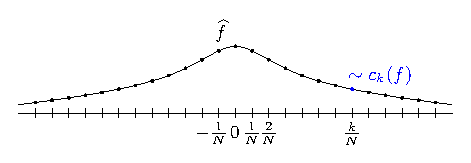
\includegraphics[width=0.55\textwidth]{MA3L29_2.eps}
	\label{MA3L29_2}
	\caption{График преобразования Фурье $\fourt{f}$, коэффициенты Фурье находятся на графике.}
	\label{fig: Преобразоване Фурье}
\end{figure}
Смотрим значения в точках на графике: это и есть, с точностью до множителя $\tfrac{1}{\sqrt{2\pi}N}$, коэффициенты Фурье. То есть оказывается, что если раскладываем функцию с компактным носителем на разных отрезках $[-N\pi,N\pi]$, то зная преобразование Фурье мы можем смотреть как устроены коэффициенты Фурье на таких отрезках.
Причем, чем больше возьмем $N$, тем сильнее можно будет подменить коэффициенты визуально на график функции. В результате получаем, что преобразование Фурье содержит в себе все возможные коэффициенты Фурье для таких функций $f$.

\begin{prop}
	Если $f$ абсолютно интегрируема на $\MR$, то есть:
	$$
		\ddint{-\infty}{+\infty}|f(x)|dx < \infty
	$$
	то преобразование Фурье существует, является непрерывной функцией и верна оценка:
	$$
		\left|\wht{f}(y)\right| \leq \dfrac{1}{\sqrt{2\pi}}\ddint{-\infty}{+\infty}|f(x)|dx
	$$
\end{prop}
\begin{rem}
	Благодаря оценке выше мы можем сказать, что преобразование Фурье в утверждении является ещё и заведомо ограниченной функцией.
\end{rem}
\begin{proof}
	Рассмотрим преобразование Фурье как несобственный интеграл с параметром и воспользуемся признаком Вейерштрасса:
	$$
		\left|\widehat{f}(y)\right| = \left|\dfrac{1}{\sqrt{2\pi}}\ddint{-\infty}{+\infty}f(x)e^{-ixy}dx\right| \leq \dfrac{1}{\sqrt{2\pi}}\ddint{-\infty}{+\infty}\left|f(x)e^{-ixy}\right|dx \leq \dfrac{1}{\sqrt{2\pi}}\ddint{-\infty}{+\infty}\left|f(x)\right|dx < \infty
	$$
	Таким образом, мы получили оценку сверху на преобразование Фурье, интеграл сходится равномерно по $y \Rightarrow$ все определено, можем переходить к пределу под интегралом: 
	$$
		\lim\limits_{y \to y_0}\wht{f}(y) = \dfrac{1}{\sqrt{2\pi}}\ddint{-\infty}{+\infty}f(x) \lim\limits_{y \to y_0} e^{-ixy}dx = \wht{f}(y_0)
	$$
	Значит интеграл получается непрерывной функцией по $y$. 
\end{proof}

\subsection*{Пространство Шварца быстроубывающих функций}
Дальнейшие общие рассуждения про преобразование Фурье в правильной общности можно будет сделать только используя материал дальнейших курсов, сейчас же это просто невозможно. 

С другой стороны, хотелось бы понять в каком естественном пространстве живет преобразование Фурье. Если выбрать правильно пространство, то с него можно будет потом перенести преобразование на очень общие функции. Таким пространством оказалось пространство Шварца (обозначаем через $S$).

\begin{defn}
	\uwave{Пространством быстроубывающих функций Шварца} назовем пространство функций:
	$$
		S = \left\{f \colon \MR \to \MC, \, f \in C^{\infty}(\MC), \, \forall m, n \in \MN \cup\{0\}, \, \sup\limits_{x 
		\in \MR}\left(1 + |x|^n\right){\cdot}|f^{(m)}(x)| < \infty\right\}
	$$
	где под $f \in C^{\infty}(\MC)$ мы понимаем бесконечную дифференцируемость функции $f$: то есть действительные и мнимые части - бесконечно дифференцируемые функции. 
\end{defn}
Из определения видно, что $f \in S$ и всякая её производная на бесконечности стремятся к нулю быстрее любой степени.

\newpage
\textbf{Примеры}: $f \equiv 0 \in S$, гладкие финитные функции $\in S$, $e^{-x^{2k}} \in S$, $P(x)e^{-x^{2k}} \in S$. 

Очевидно, что $S$ - линейное пространство над $\MC$. Более того, $S$ - алгебра, поскольку: 
$$
	f,g \in S \Rightarrow f{\cdot}g \in S
$$
Функция бесконечно гладкая $\Rightarrow$ производная будет бесконечно гладкой, если любая производная стремилась быстрее степени $\Rightarrow$ у производной будет то же свойство:
$$
	f \in S \Rightarrow f^{(k)} \in S
$$ 
Отсюда можно получить простое следствие:
$$
	f \in S, \, P - \text{многочлен} \Rightarrow P{\cdot}f \in S
$$
то есть этот класс функций выдерживает умножение на многочлены. Нашей целью будет показать, что преобразование Фурье является линейным изоморфизмом пространства $S$. Часто распространение преобразования Фурье на другие пространства начинается именно с $S$.
\begin{theorem}(\textbf{преобразование Фурье и дифференцирование}) $\forall f \in S$ будут верны следующие соотношения:
	$$
		\fourt{f^{(k)}}(y) = (iy)^k\fourt{f}(y)
	$$
	$$	
		\fourt{f}^{(k)}(y) = \fourt{(-ix)^kf(x)}(y)
	$$
\end{theorem}

\begin{proof}
	Поскольку $f$ из $S$, то все интегралы существуют. Тогда воспользуемся интегрированием по частям:
	$$
		\fourt{f^{(k)}}(y) =  \dfrac{1}{\sqrt{2\pi}}\ddint{-\infty}{+\infty}f^{(k)}(x)e^{-ixy}dx = iy\dfrac{1}{\sqrt{2\pi}}\ddint{-\infty}{+\infty}f^{(k-1)}(x)e^{-ixy}dx = \dotsc = (iy)^{k}\fourt{f}(y)
	$$
	$$
		\fourt{(-ix)^kf(x)}(y) = \dfrac{1}{\sqrt{2\pi}}\ddint{-\infty}{+\infty}(-ix)^kf(x)e^{-ixy}dx = \dfrac{1}{\sqrt{2\pi}}\ddint{-\infty}{+\infty}f(x){\cdot}\dfrac{d^k}{d y^k} (e^{-ixy})dx	= 
	$$
	$$	
		= \dfrac{d^k}{d y^k}	\dfrac{1}{\sqrt{2\pi}}\ddint{-\infty}{+\infty}f(x)e^{-ixy}dx = \fourt{f}^{(k)}(y)
	$$
	где мы применили теорему о дифференцировании интеграла с параметром. Для этого необходимо проверить сходимость интеграла:
	$$
		f(x) \in S \Rightarrow \left|\ddint{-\infty}{+\infty}f(x)e^{-ixy}dx \right| \leq \ddint{-\infty}{+\infty}|f(x)|dx < \infty \Rightarrow \dfrac{1}{\sqrt{2\pi}}\ddint{-\infty}{+\infty}f(x)e^{-ixy}dx < \infty
	$$
	Также необходимо проверить второе, что после дифференцирования сходимость - равномерная. Продифференцируем:
	$$
		\left(\ddint{-\infty}{+\infty}f(x)e^{-ixy}dx\right)' = \dfrac{1}{\sqrt{2\pi}}\ddint{-\infty}{+\infty}(-ix)f(x)e^{-ixy}dx \Rightarrow  \left|\ddint{-\infty}{+\infty}(-ix)f(x)e^{-ixy}dx\right| \leq \ddint{-\infty}{+\infty}|x|{\cdot}|f(x)|dx < \infty
	$$
	Поскольу $xf(x) \in S$ (оценка сверху), то мы получаем равномерную сходимость.
\end{proof}
\begin{rem}
	Особенность этого утверждения заключается в том, что преобразование Фурье превращает дифференцирование в умножение на степень (с точностью до $i^k$) и наоборот умножение на степень превращает в дифференцирование. А поскольку обещано, что преобразование Фурье будет линейным изоморфизмом, то это замена базиса, в которой дифференцирование превращается в умножение.
\end{rem}

\begin{corollary}
	Преобразование Фурье отображает $S$ в $S$
\end{corollary}

\begin{rem}
	В следующий раз мы отметим, что преобразование Фурье это линейное отображение, значит $S$ это инвариантное подпространство для этого оператора.
\end{rem}

\end{document}